\section{Materials and Methods}\label{s:3}

\subsection{System Overview}

\begin{figure}[htb]
    \centering{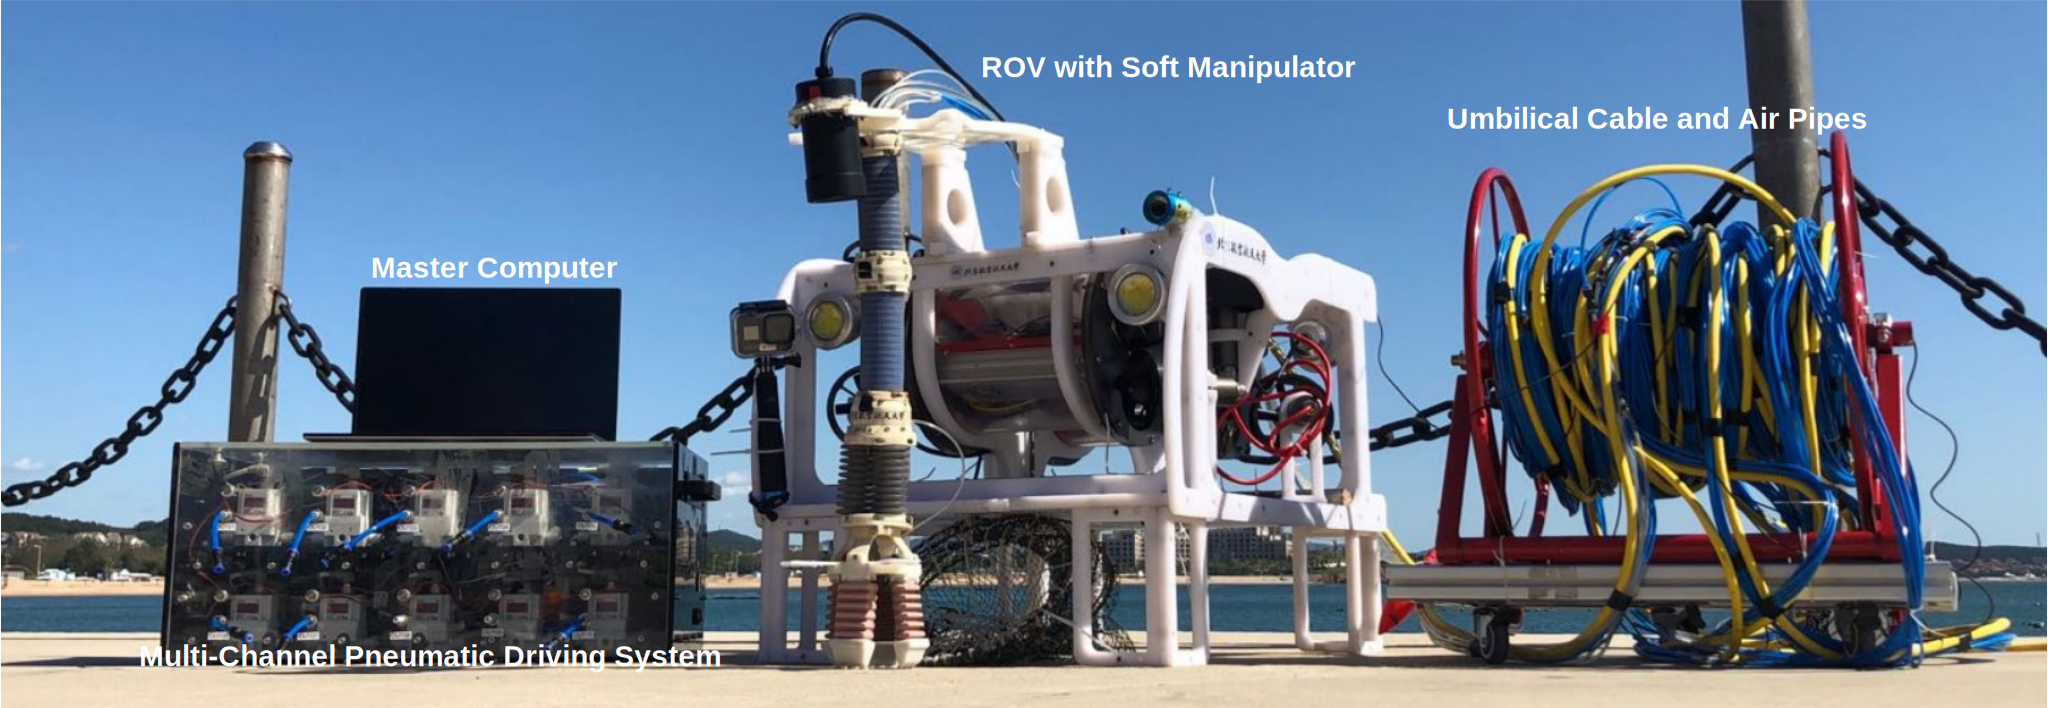
\includegraphics[width=\textwidth]{Figures/overview.pdf}}
    \caption[Autonomous seafood grasping system overview]{Autonomous seafood
        grasping system overview: a modified \gls{rov}, an \gls{OBSS} soft
        manipulator and a master computer}\label{f:overview}
\end{figure}

As shown in~\autoref{f:overview}, the auto seafood grasping system consists of a
modified \gls{rov}, an \gls{OBSS} soft manipulator, a multi-channel pneumatic
driving system and a master computer. The \gls{OBSS} soft manipulator is
installed vertically down and was controlled to pick-and-place seafood into a
collecting basket fixed to the bottom front of the \gls{iauv}. A modified
4-\gls{dof} (forward/backward, left/right, up/down, spin) \gls{rov} is
integrated with a binocular camera \citetitle{zed} for cruise and target
detection, which placed with an angle to vertical down direction, and a fishing
camera to provide a wider view to monitor the whole working environment. These
two cameras are connected to the control unit of the \gls{iauv}, where the video
stream from the binocular camera was processed. The processed binocular camera
video stream together with video stream from the fishing camera were sent to the
master computer onboard the vessel by \gls{rtsp} though a local network. There,
on the master computer low latency monitoring and controlling of the \gls{iauv}
in emergent situations were allowed. The \gls{iauv} measures 600 mm long, 500 mm
wide, and 300 mm tall, with a weight of approximately 30 kg and an operating
depth of 0{-}50 meters.

\subsection{Hardware}

\subsubsection{Design of the Vehicle}

\begin{figure}[htb]
    \centering{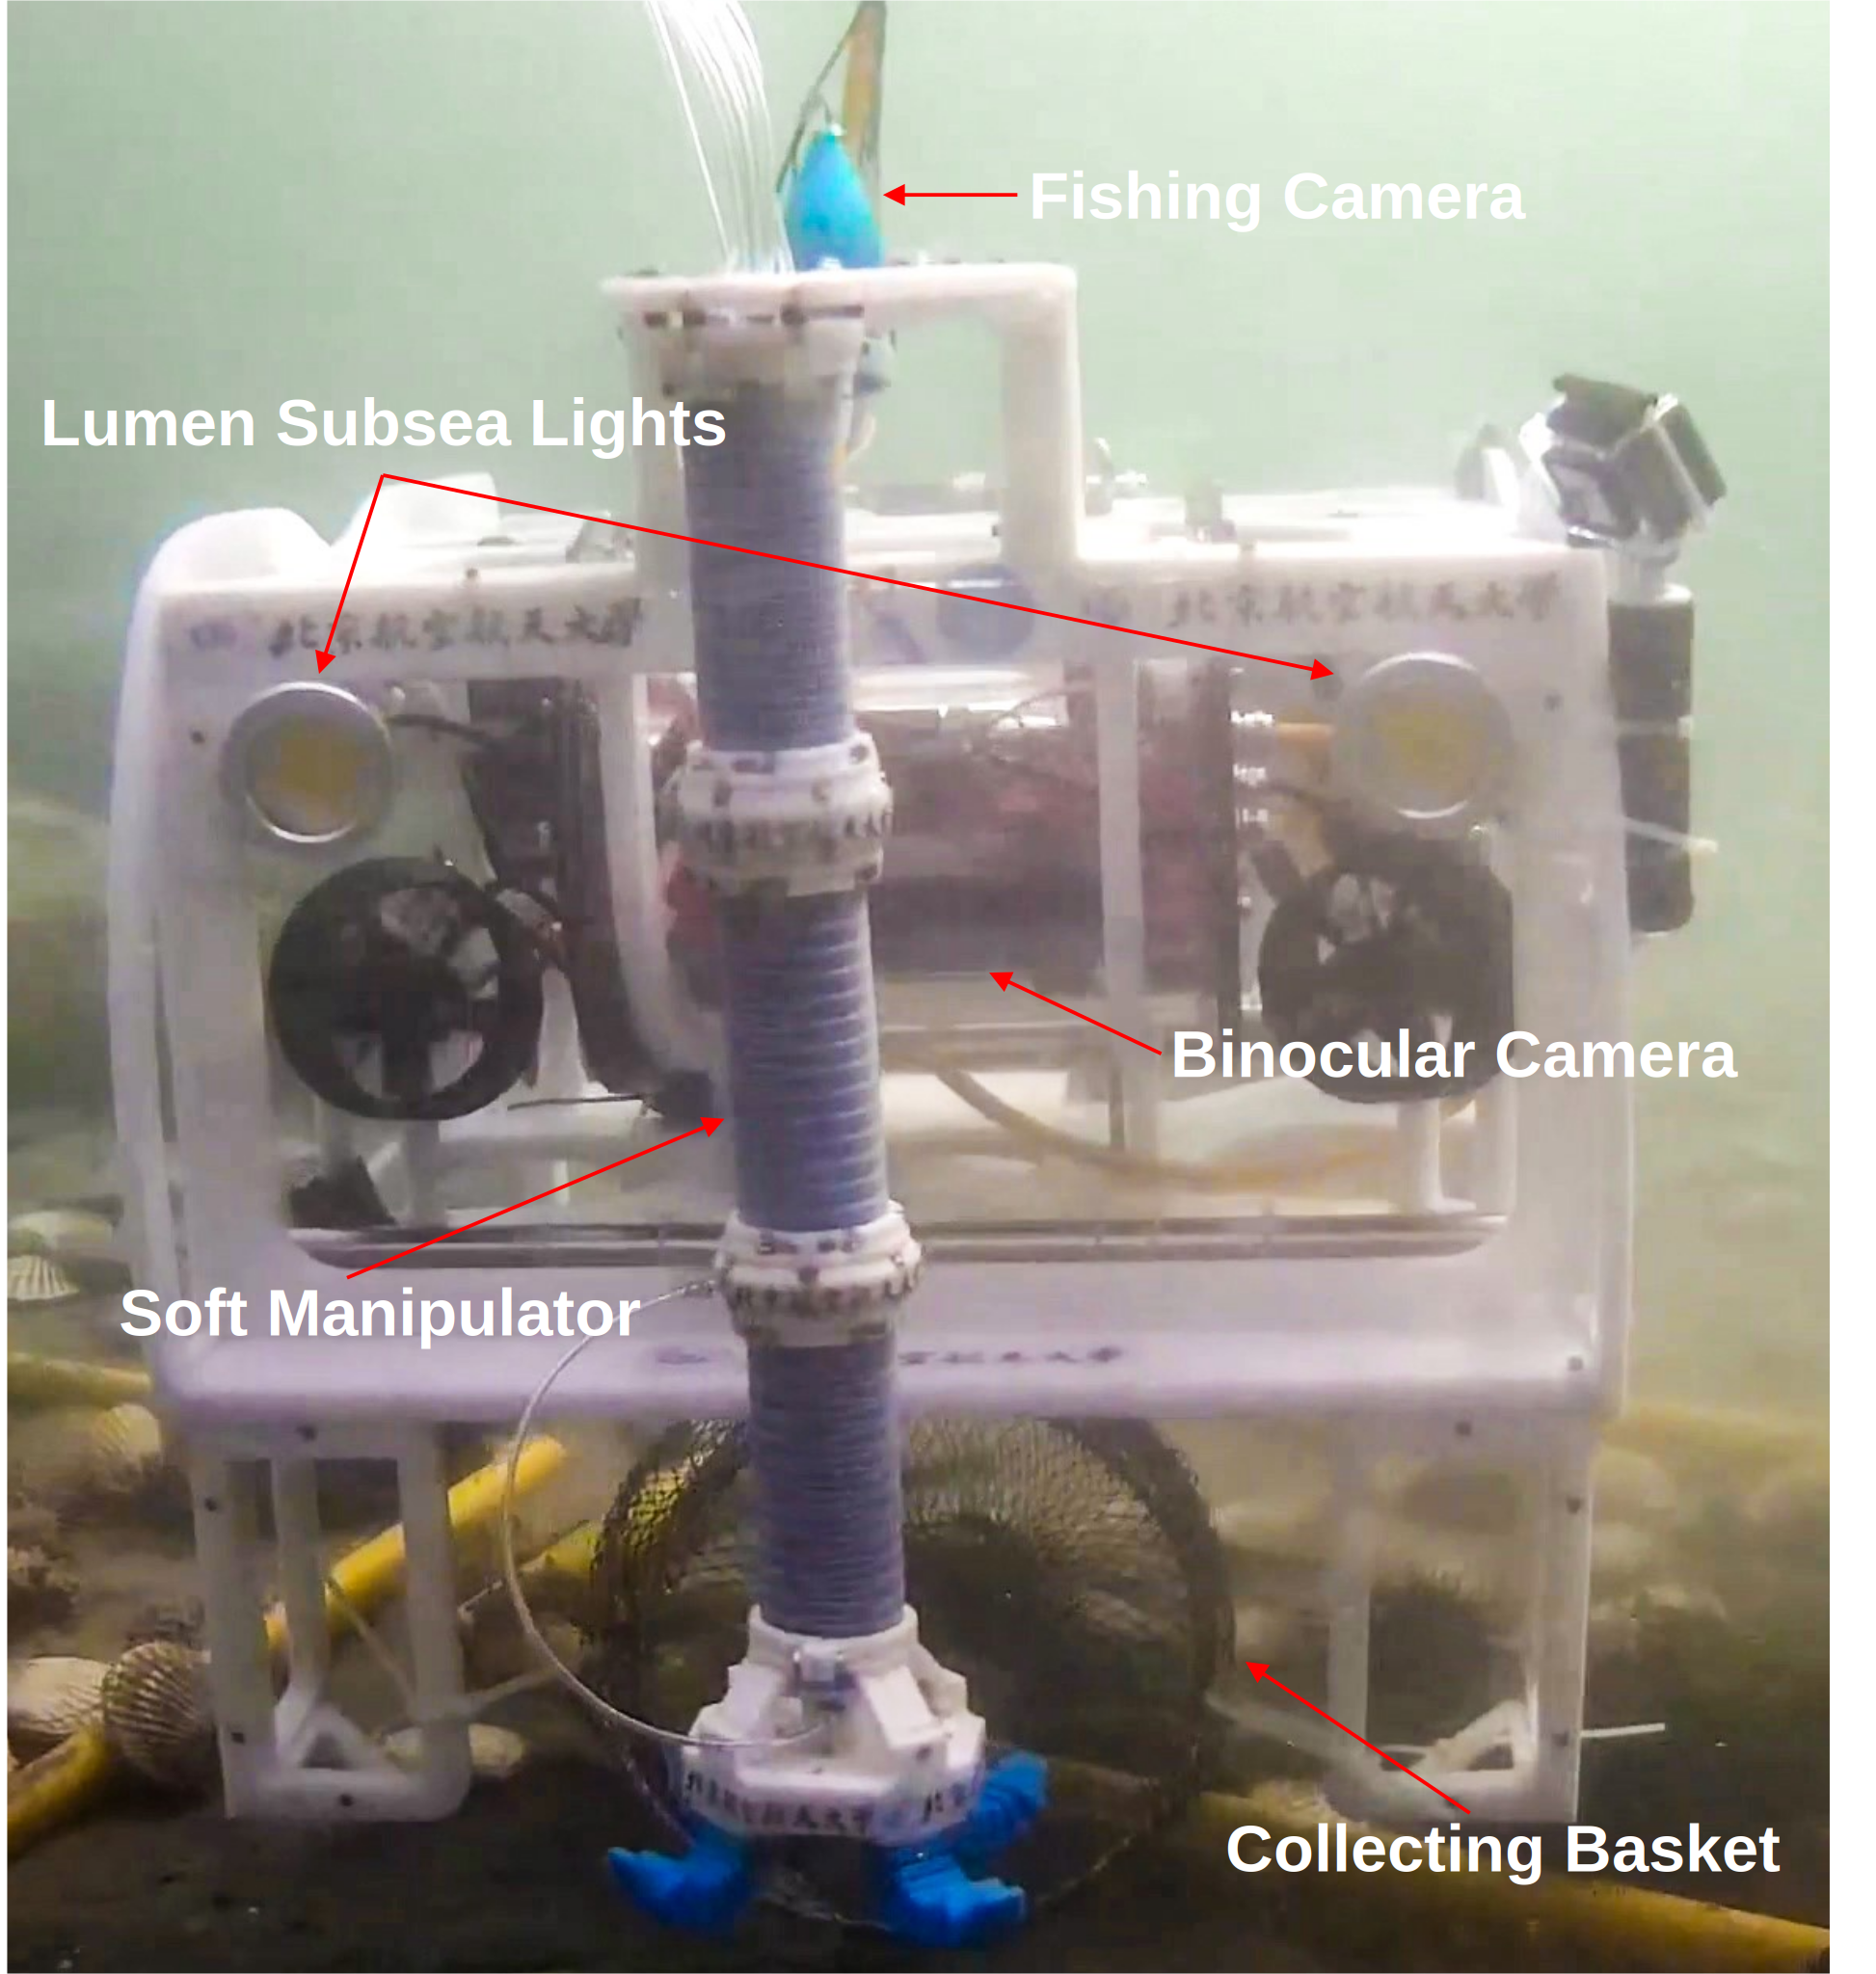
\includegraphics[width=0.8\textwidth]{Figures/vehicle.pdf}}
    \caption[Vehicle components]{Vehicle components: snapshot of the underwater
        robot system with a soft manipulator for grasping fragile sea
        animals.}\label{f:vehicle}
\end{figure}

The entire vehicle is visualized in \autoref{f:vehicle}.The vehicle is in shape
of \ensuremath{600 mm \times 500 mm \times 300 mm}, weighing around 30kg,
consist of the frame, a depth sensor, a propulsion system, four LED lights, a
binocular camera, a fishing camera, two sealed warehouse and a collecting
basket. The white frame are assembled laser-cut \gls{pmma} boards with thickness
of about 1 cm, fixed to each other with at least four screws. This structure
guarantees stability of the robot under any circumstances in the depth range of
0{-}50 meters. \gls{pmma} could gain substantial amount of buoyancy whether in
lab pool condition or submarine condition, in the meanwhile, huge hollowed-outs
are applied to the design, both of which helped to reduce the total weight of
the vehicle. The natural light condition at more than 10 meters below sea level
could be horrible for target detection by \gls{cv}. Therefore the headlights and
taillights were applied to provide supplementary lighting to enhance the quality
of images captured by the binocular camera and fishing camera. Two column-shaped
sealed warehouse were loaded inside the vehicle. The front warehouse contained a
communication unit including a ethernet-to-fiber converter, power unit and the
back warehouse contained a control unit, a 6-channel motor driver. The
thrusters, depth sensor, two cameras, four lights are all connected to the
control unit (\autoref{f:topology}).

\begin{figure}
    \centering{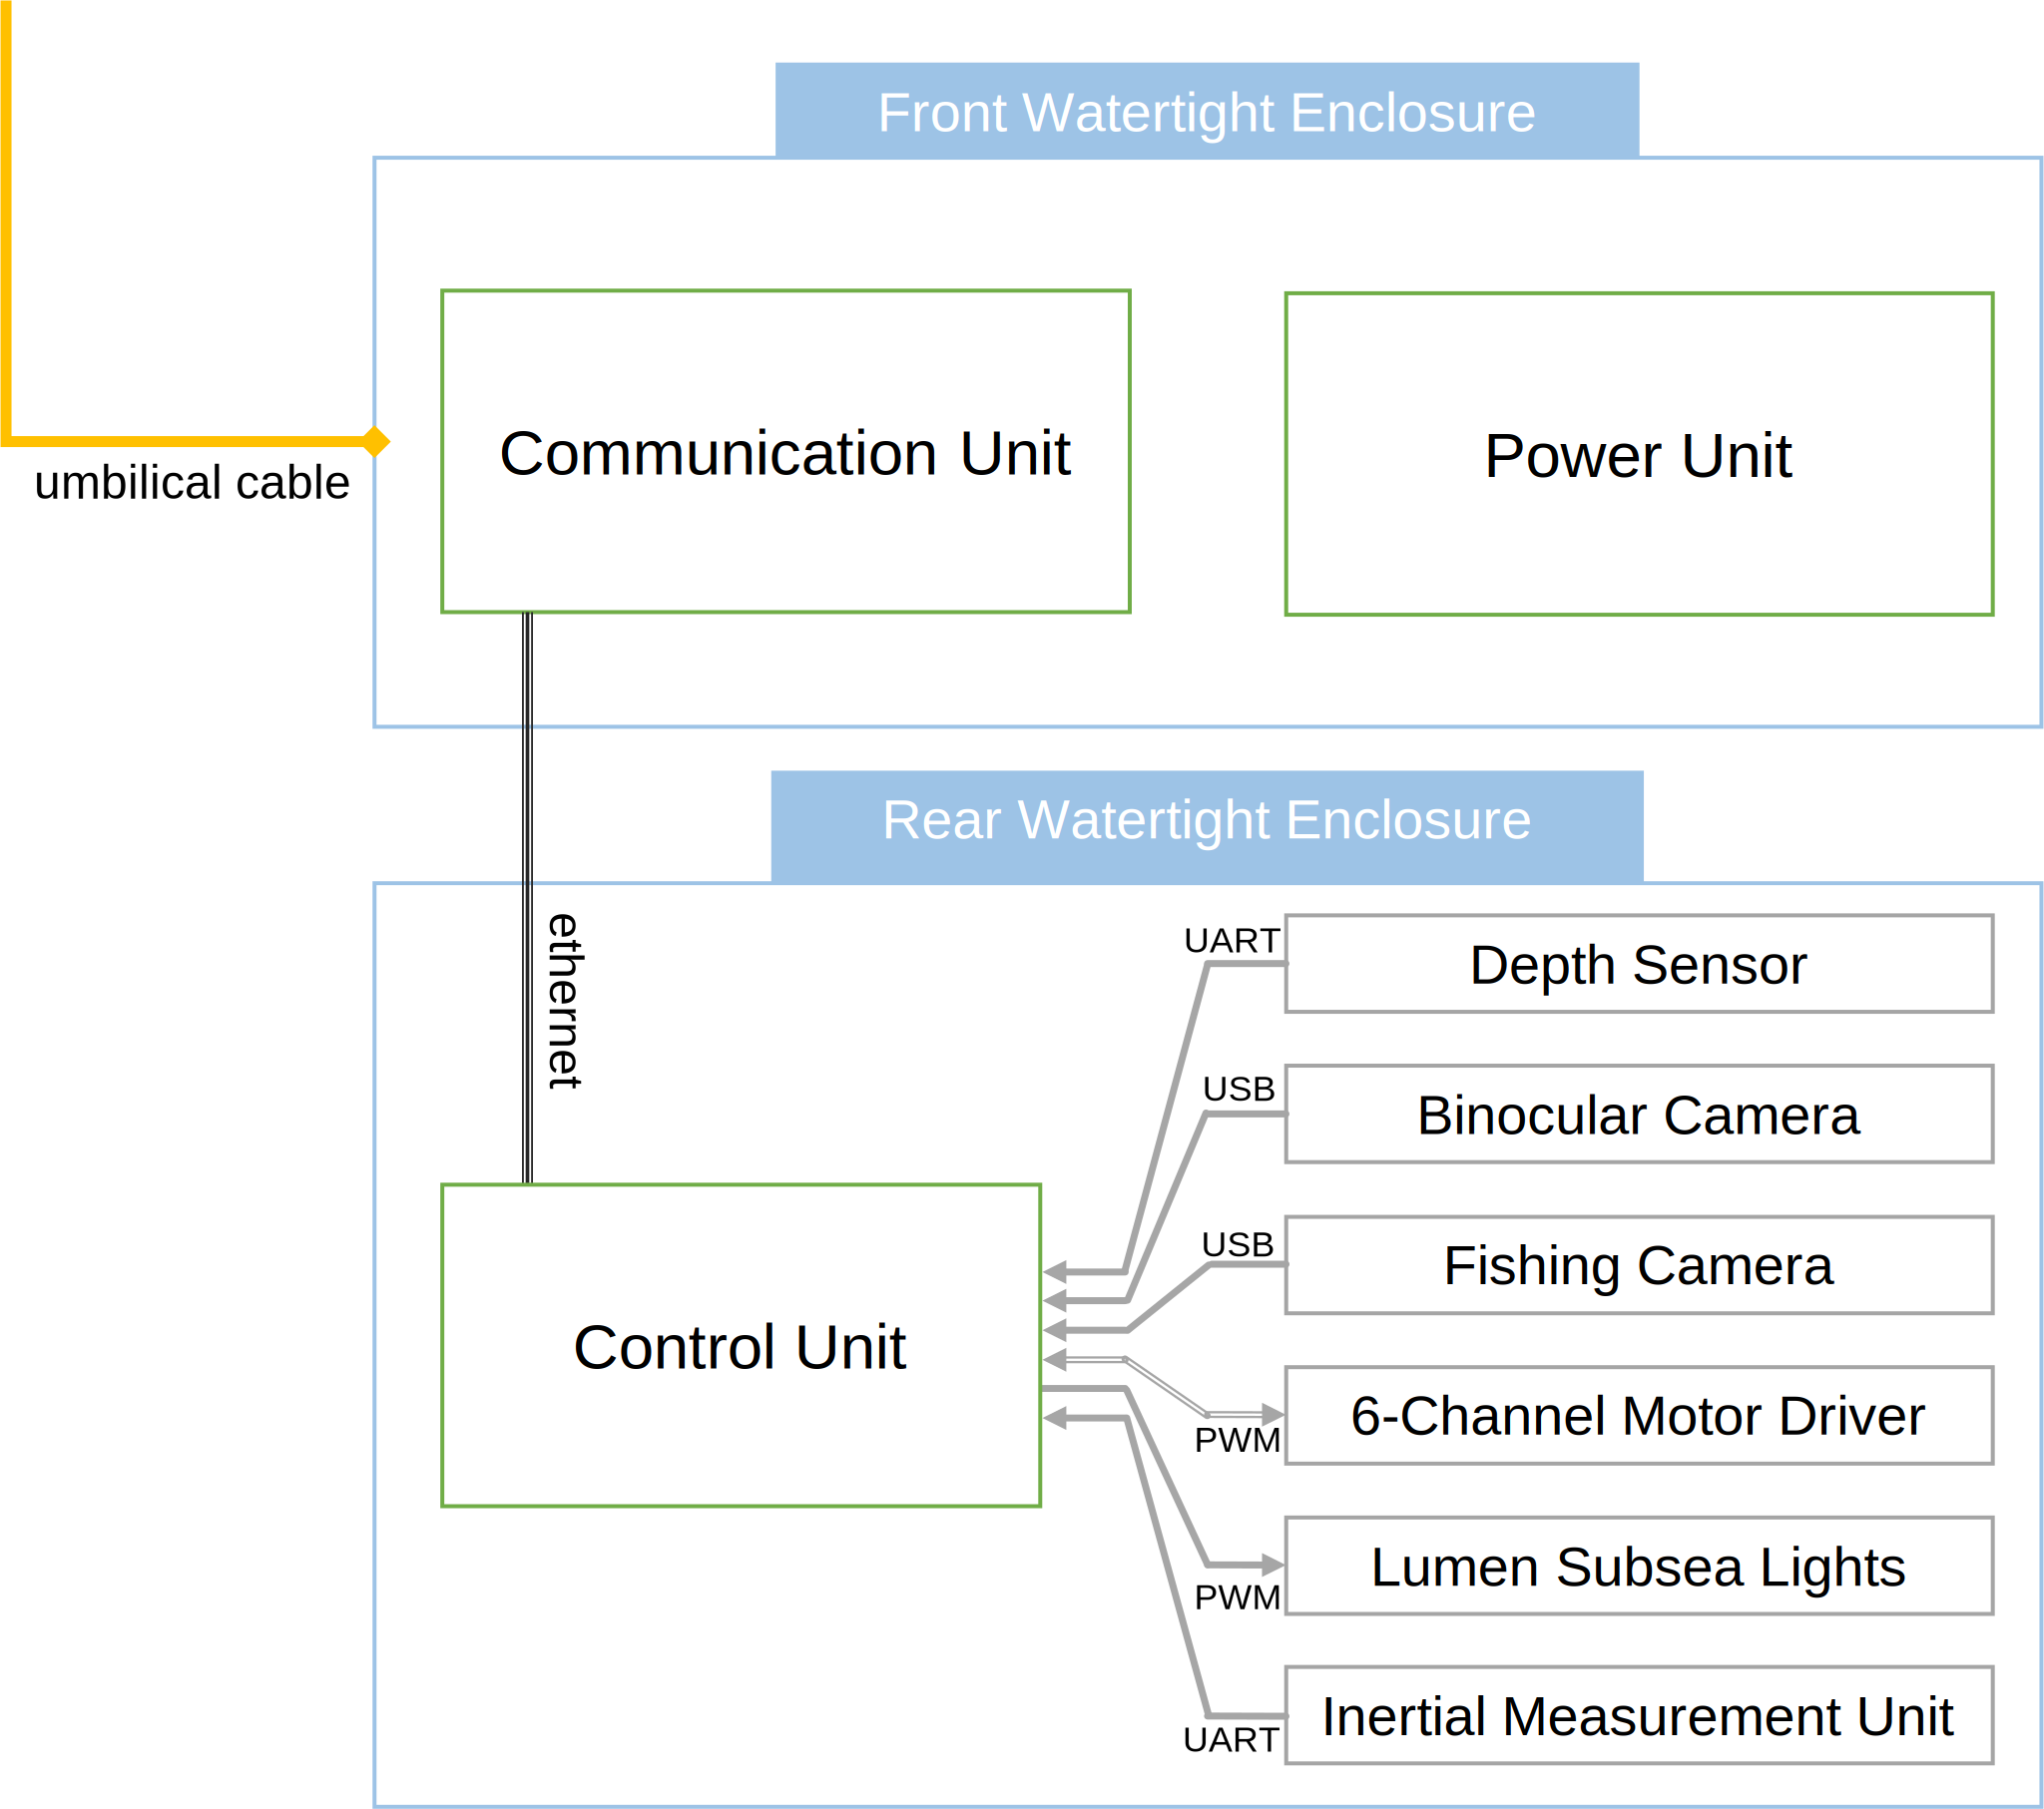
\includegraphics[width=0.7\textwidth]{Figures/topology.pdf}}
    \caption[Device topology]{Device topology: topology of all modules and
        devices integrated on the vehicle}\label{f:topology}
\end{figure}

\paragraph{Depth Sensor}

The depth sensor is placed near the bottom of the vehicle with its working
surface downward, which direction proved to obtain minimum noise (less than 3 mm
in most experiments) caused by the oceanic current. The depth is deduced from

\begin{equation}
    h_d = \frac{P_d - P_0}{\gls{rhoe} \gls{g}}
\end{equation}

where \ensuremath{P_d} is the current pressure detected by the sensor,
\ensuremath{P_0} is the initial pressure detected when the sensor was powered
up, \ensuremath{\rho_e} is the underwater environment density (\ensuremath{1,025
    kg/m^3} is considered as the seawater density), and \ensuremath{h_d} is the
current depth.

With accuracy of no more than 3 mm in most experiments, the precise of this
depth sensor could definitely meet the specification required by tasks in this
project.

\paragraph{Propulsion System}

Designed similar to a quadrocopter, the propulsion system of this \gls{iauv}
consists of 6 thrusters, four of which are placed at right the same level of the
mass center, in charge of horizontal movements, and the other two are placed
symmetric about the centerline, in charge of vertical movements
(\autoref{f:propulsion}). By keeping four horizontal movements thrusters at the
same level of the mass center and symmetric against the center, when thrust
forces are applied, there won't be torques generated against water resistance.
The driving force provided by this propulsion system is actually not enriched
for high mobility required by the complex operating condition. The max speed of
forward/backward movement is approximately \ensuremath{2.5 m/s} and max speed of
side movement and vertical movement is approximately \ensuremath{2 m/s}.

Speed of the motors were regulated with \gls{pwm}, which basically controls the
high level time of voltage supplied to the motors in a period (called duty
cycle), with resolution of 256 levels (including forward and reverse rotation).
Provided this technique, control of motor speed, from stop to full speed,
through analog voltage supplied to the motors simply with an 8-bit digital input
is allowed. Meanwhile, the voltage supplied to each motor is detected and
recorded as sensor signals in real-time.

\begin{figure}[htb]
    \centering{\includegraphics[width=\textwidth]{Figures/propulsion.pdf}}
    \caption[Propulsion system]{Propulsion system: (a) four thrusters for
        horizontal moving. (b) two thrusters for vertical
        moving}\label{f:propulsion}
\end{figure}

\paragraph{Control Unit}

The flow of signals within the control unit is depicted in \autoref{f:cu}. The
control unit is actually made up of two boards: a \citetitle{jetson} for
top-level control and a \citetitle{stm32} for low-level control. The
\citetitle{jetson} is connected to the local network through ethernet, able to
send required pressure values to the multi-channel pneumatic driving system as
well as send data packages of video streams and data from sensors integrated on
the vehicle to the master computer at about 20 \gls{fps} (and may receive
commands from the master computer in emergent situations). In the meanwhile the
\citetitle{stm32} could only communicate with the \citetitle{jetson}, receiving
commands and transmitting data from sensors. Possible commands and sensor
signals are listed in \autoref{t:stm32}.

\begin{table}[htb]
    \renewcommand*{\arraystretch}{1.3}
    \centering
    \begin{tabularx}{0.8\textwidth}{XX}
        \toprule
        \textbf{Possible commands} & \textbf{Possible sensor signals}        \\
        \midrule
        lights on/off              & depth of the vehicle, \gls{hd}          \\
        move upwards/downwards     & voltage supplied to each motor          \\
        move forwards/backwards    & pitch angle of the vehicle, \gls{pitch} \\
        move leftwards/rightwards  & roll angle of the vehicle, \gls{roll}   \\
        turn left/right            & yaw angle of the vehicle, \gls{yaw}     \\
        \bottomrule
    \end{tabularx}
    \caption[Possible Commands and Sensor Signals for STM32 board]{Possible
        commands sent to the \citetitle{stm32} and possible sensor signals from it
        (left column and right column were not correspondent)}\label{t:stm32}
\end{table}

An 6-\gls{dof} \gls{imu} (composed of a 3-axis accelerometer and a 3-axis
gyroscope) is integrated on the board of \citetitle{stm32}. Both the
acceleration information and angular velocity are used to enhance the movement
control of the vehicle, but only Euler angles deduced by the angular velocities
are sent to \citetitle{jetson} as signals. \citetitle{stm32} kept sending
digital signals to the 6-channel motor driver and 4-way lights at a rate of 30
Hz with resolution of 256 levels and 960 levels respectively, until new command
received from the \citetitle{jetson}.

A \gls{rtsp} server was established on the \citetitle{jetson} to publish live
video streams from the \citetitle{zed} and fishing camera into the local
network. This technique allow any device in the local network to get access to
view from \citetitle{zed} or the fishing camera through whether browser, player
like vlc or self-developed application with \gls{rtsp}.

\begin{figure}[htb]
    \centering{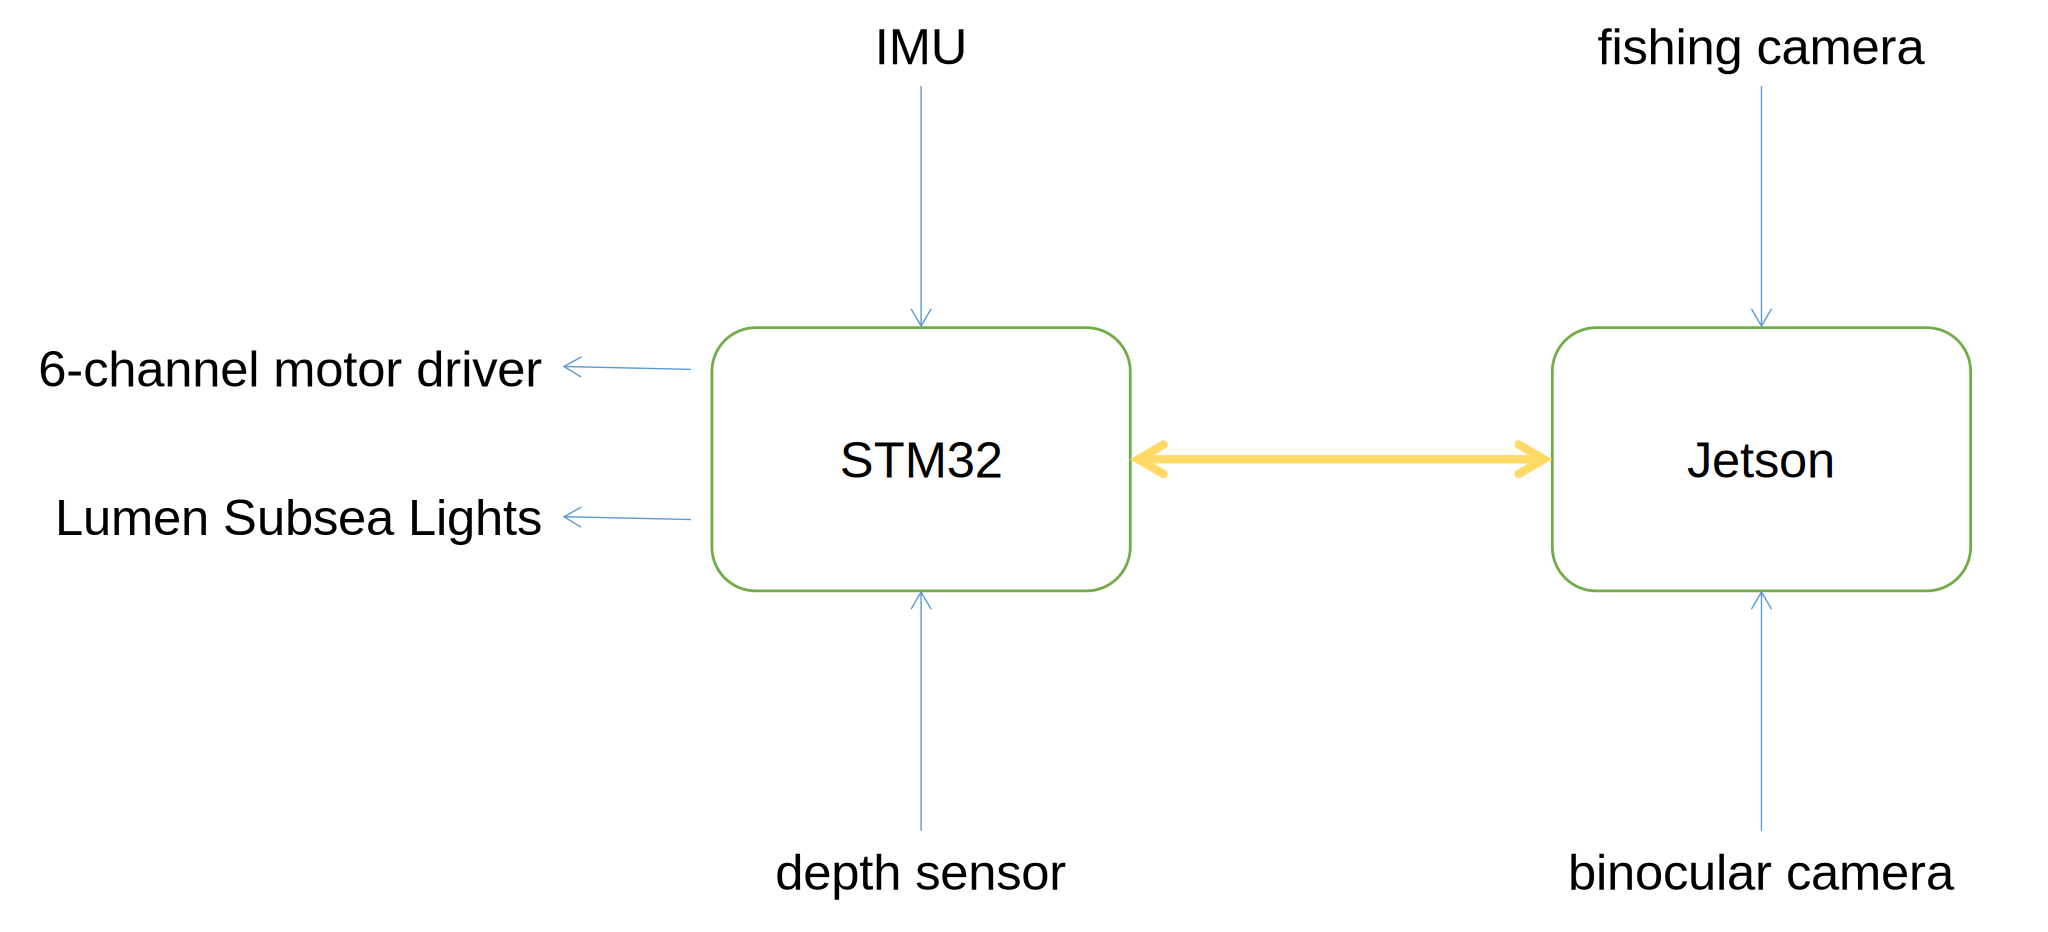
\includegraphics[width=0.8\textwidth]{Figures/cu.pdf}}
    \caption[Control Unit]{Control Unit: Block diagram of signal flow inside the
        Control Unit}\label{f:cu}
\end{figure}

\paragraph{Binocular Camera}

The \citetitle{zed} binocular camera is placed at the front of the vehicle,
about the level of the vehicle's center (\autoref{f:vehicle}), to get a relatively close view spanning
the workspace of the manipulator's end effector. For such purpose, there is an
angle of 30 degrees between the direction of the camera and the vertical
downward direction. \citetitle{zed} is not waterproof by itself, so a 3D-printed
waterproof cage is introduced to provide resistance to submersion up to a
maximum depth of 30 meters underwater (\autoref{f:zed}).

\begin{figure}[htb]
    \centering{\includegraphics[width=0.9\textwidth]{Figures/zed.jpg}}
    \caption[Side View of ZED with waterproof cage]{Side view of \citetitle{zed}
    with waterproof cage}\label{f:zed}
\end{figure}

\subsubsection{Design and Actuation of the Soft Robotic Manipulator}

An three segments \gls{OBSS}  underwater soft manipulator was integrated onto
the vehicle and used to grasp and place targets into the basket
(\cite{gong2021soft}). As indicated in \autoref{f:manipulator}, the manipulator
consisted of two bending segments, a stretching segment and a soft gripper. The
manipulator was actuated with an opposing curvature where
\(\gls{theta1}=\gls{theta2}\). The two bending segments had a joining angle of
180 degrees. In this assembling pattern, for instance, chamber\ballnumber{1} of
the upper bending segment is in the opposite position to chamber\ballnumber{1}
of the lower bending segment, where the intersection angle is 180 degrees.

\begin{figure}[htb]
    \centering{\includegraphics[width=\textwidth]{Figures/manipulator.jpg}}
    \caption[Design and Mechanics of the Underwater Soft Manipulator]{Design and
    mechanics of the underwater soft manipulator: (a) An overview of the
    \gls{OBSS} soft manipulator (scale bar 50 mm). (b) Components of the
    manipulator with annotations of useful magnitudes. (c) An illustration of
    how chambers  are arranged in the two bending segments. (d) A closer view of
    the upper end of the stretching segment.}\label{f:manipulator}
\end{figure}

\subsection{Software}

Programs ran in this autonomous grasping system could be defined as three
modules: slave low-level module written in C++, slave high-level module written
in C++ and master module written in Python, on the \citetitle{stm32},
\citetitle{jetson} and master computer respectively. Most computational tasks
were done in the slave high-level module by the \citetitle{jetson}, which
brought supercomputer performance (almost same compute capability of a GeForce
RTX 2080 desktop version, \autocite{cc}) to the edge. This module is in charge
of a series of tasks which requires relatively high performance listed below:

\begin{itemize}
    \item keeps pushing video streams from two cameras into the local network
          with \gls{rtsp} once its system was started up
    \item realtime underwater vision restoration of video stream from the
          binocular camera, to enhance quality of the images
    \item realtime target (sea cucumber, sea urchin or scallop) detection and
          tracking from the latest frame from the binocular camera
    \item realtime target distance estimation with depth map deduced by
          \gls{sgbm} algorithm (triggered if target detected)
    \item realtime ARUCO marker detection (triggered if grasping started)
\end{itemize}

Main configurations of the \citetitle{jetson} and software environment used for
\gls{cv} in this project can be found in \autoref{a:cvconfig}.

\subsubsection{AUV Movement Control}

The speed on each directions are regulated by a 6-way \gls{pid} controller on
the \citetitle{stm32}. The tunning of the controller was done with the
Ziegler-Nichols method (\cite{aastrom2004revisiting}). In addition, The depth of
the \gls{iauv} were also under \gls{pid} control, which enables hovering stably
in underwater environment with small current.

As shown in \autoref{f:propulsion}, 6 thrusters are used to provide movements
listed in. To simplify the kinematics model (therefore improves the robustness),
turing and orientational moving at the same time is not allowed. How thrusters
perform when doing horizontal movements are shown in \autoref{t:thruster}.
Besides, thruster 5 and thruster 6 were always working with the same direction
of rotation, rotating clockwise to move upward and rotating anticlockwise to
move downward.

\begin{table}[htb]
    \renewcommand*{\arraystretch}{1.3}
    \centering
    \begin{tabularx}{\textwidth}{Xcccc}
        \toprule
        movement                                                    & left front thruster & right front thruster & left rear thruster & right rear thruster \\
        \midrule
        \(\uparrow\) forward                                        & \(-\)               & \(-\)                & \(+\)              & \(+\)               \\
        \(\downarrow\) backward                                     & \(+\)               & \(+\)                & \(-\)              & \(-\)               \\
        \(\leftarrow\) leftward                                     & \(-\)               & \(+\)                & \(-\)              & \(+\)               \\
        \(\rightarrow\) rightward                                   & \(+\)               & \(-\)                & \(+\)              & \(-\)               \\
        \rotatebox[origin=c]{180}{\(\circlearrowleft\)} left turn   & \(+\)               & \(-\)                & \(-\)              & \(+\)               \\
        \rotatebox[origin=c]{180}{\(\circlearrowright\)} right turn & \(-\)               & \(+\)                & \(+\)              & \(-\)               \\
        \bottomrule
    \end{tabularx}
    \caption[Movements of AUV with Status of Each Thruster for Horizontal
        Shift]{Movements of the AUV with status of each thruster for horizontal
        shift: \(+\) and \(-\) represent the positive propel (with this \gls{iauv},
        anticlockwise rotation) and reverse propel respectively}\label{t:thruster}
\end{table}

\subsubsection{underwater vision restoration and target detection}

\begin{figure}[htb]
    \centering{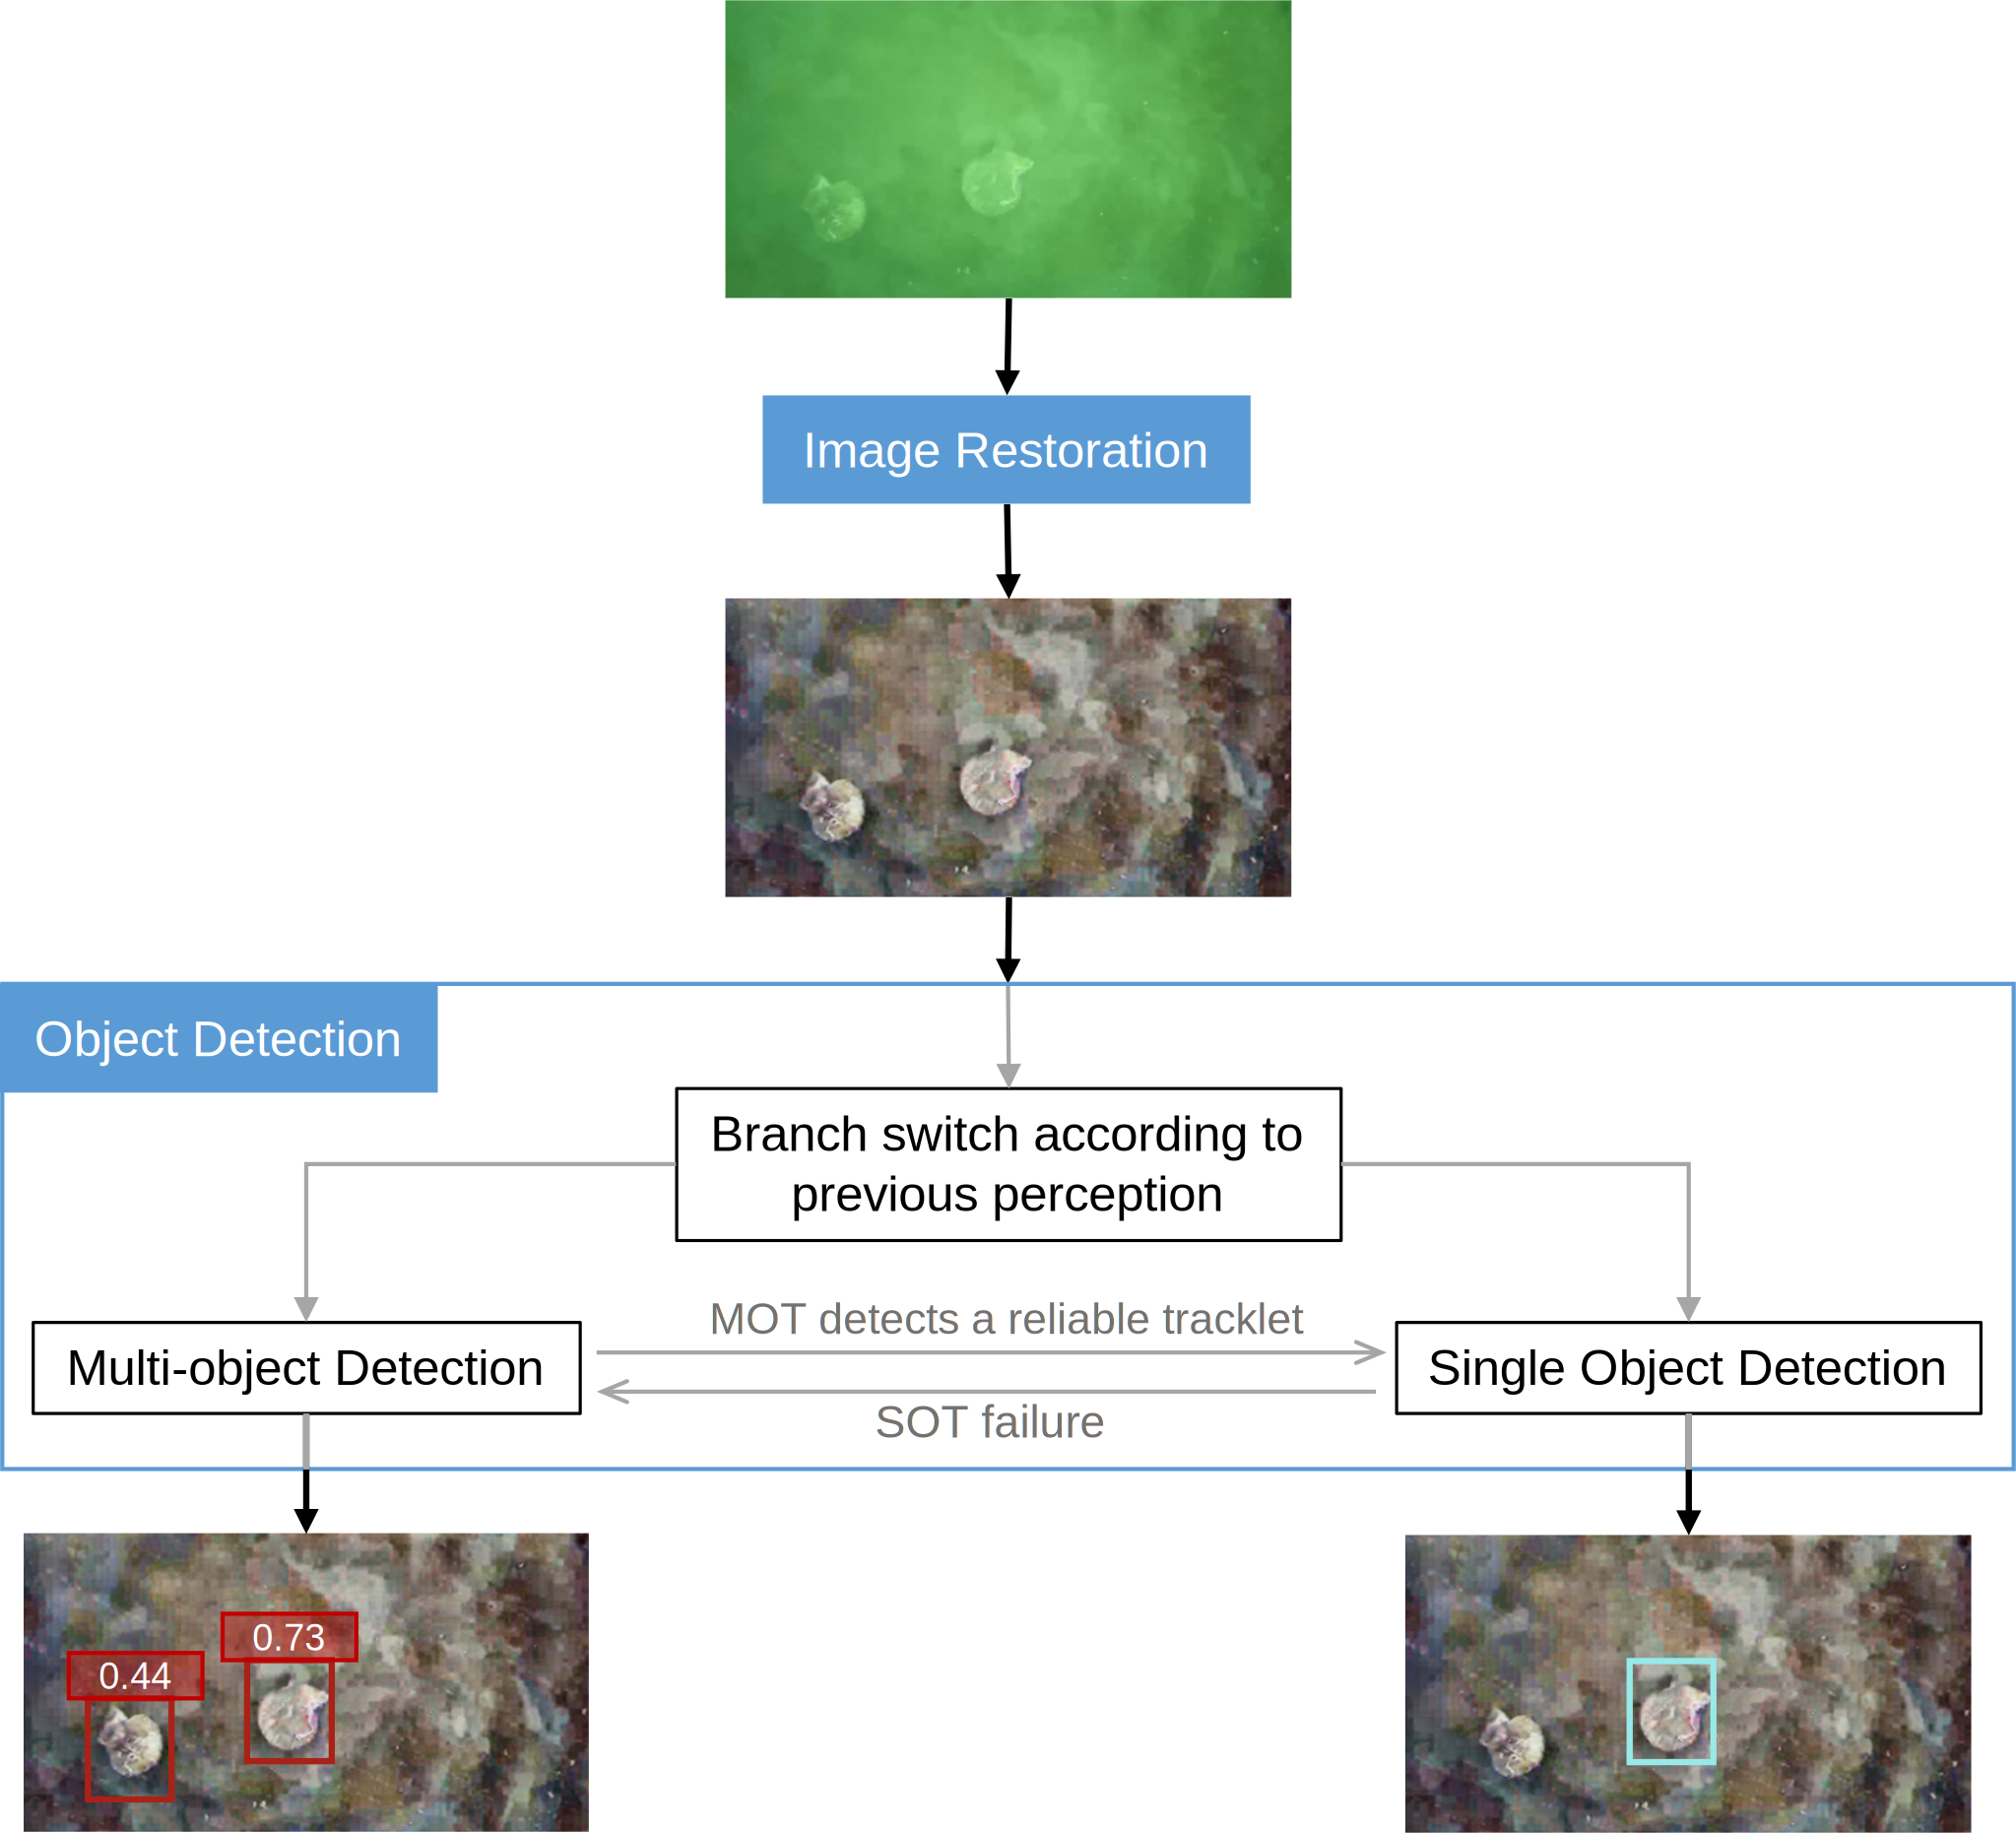
\includegraphics[width=0.9\textwidth]{Figures/detection.pdf}}
    \caption[Scheme of Underwater Seafood Detector]{Scheme of underwater seafood
        detector integrated with TSSD-OTA and GAN-RS}\label{f:detector}
\end{figure}

A real time adaptive \gls{gan}-based restoration scheme (GAN-RS)
(\cite{chen2019towards}) is integrated to enhance quality of underwater vision
and induce an overall superior restoration performance. A temporally
identity-aware \gls{ssd} with online tubelet analysis (TSSD-OTA) is used to
real-time detect and track target seafood with high performance and robustness
(\cite{chen2019temporally}). Referring to \autoref{f:detector}, the GAN-RS and
TSSD-OTA are trained into a single PyTorch model, to increase the integration
and decrease the complexity to deploy the system onto embedded device,
\citetitle{jetson} in this case, and could be called easily with libtorch (C++
\gls{api} of PyTorch).

\subsubsection{ArUco Makrer Detection}

A tiny but with high performance and strong robustness C++ library ArUco
(\cite{romero2018speeded,garrido2016generation}) is used to estimation pose of
ARUCO markers placed on the hand of the soft manipulator. With ArUco, we can get
real time position, rotation and translation of squared ARUCO markers against
the camera. Detecting and tracking of multiple markers at the same time is
supported, since an unique identifier could be decoded from the binary pattern
of every marker. Markers with size of \(5\times5\) blocks were used in this project.

\subsubsection{Communication System}

\begin{figure}[htb]
    \centering{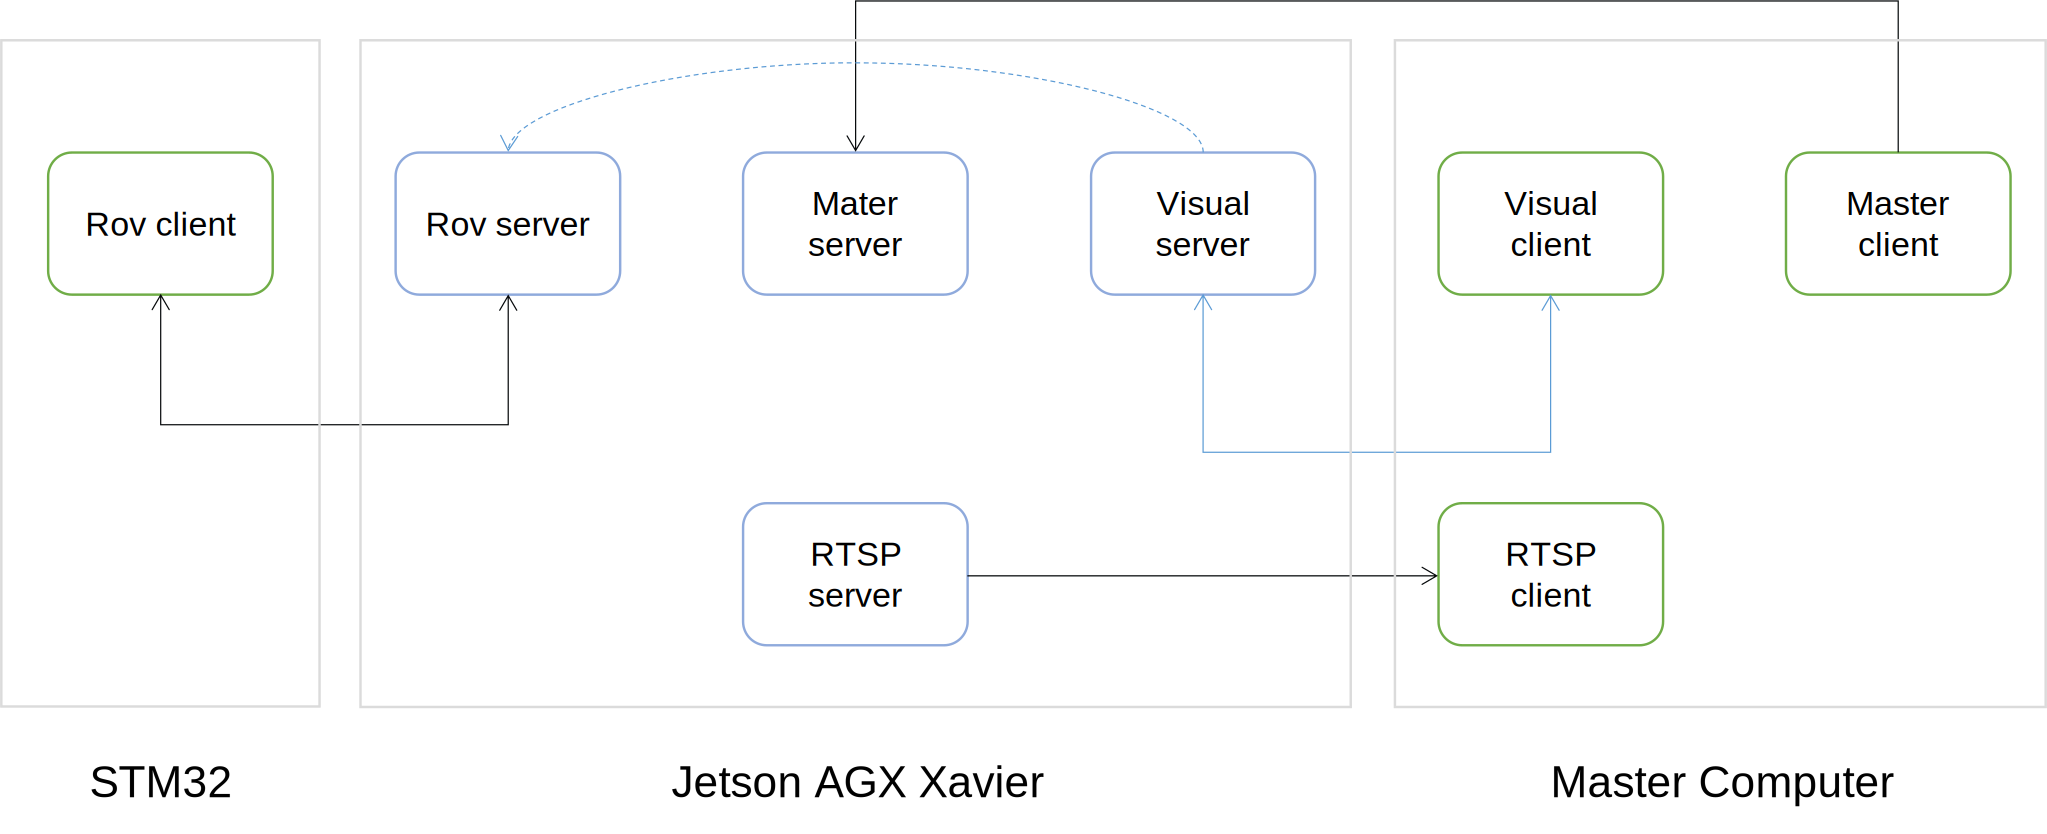
\includegraphics[width=0.9\textwidth]{Figures/communication.pdf}}
    \caption[Communication System of the Autonomous Seafood Grasping
        System]{Communication system of the Autonomous seafood grasping
        system}\label{f:communication}
\end{figure}

As illustrated in \autoref{f:communication}, there were in total 5 \gls{tcp}
socket servers and 5 correspondent \gls{tcp} socket clients in the communication
system of this autonomous seafood grasping system from 4 devices:
\citetitle{stm32}, \citetitle{jetson}, master computer and multi-channel
pneumatic driving system. Existing communication framework like ROS was not
introduced for following three reasons:

\begin{itemize}
    \item the communication system was of acceptable complexity, extra
          communication framework is not a must
    \item introducing huge frameworks may improve the robustness of
          communication, when it comes to handling unexpected situations, but more
          efforts were required to adapt the whole program to the framework used
    \item dependency of huge framework increases the workload to setup the whole
          system, especially when devices in the system spans a variety of
          architecture
\end{itemize}

As the system startup, the \citetitle{stm32} and the \citetitle{jetson} are
powered on at the same time, but the \citetitle{stm32} would start working first
since it does not have to load a operating system. So the \texttt{rov\_client}
would be the first node initialed in the system and blocked at the
\texttt{rov\_client.connect{()}}, until the \texttt{rov\_server} initialized and
started listening. The \texttt{proxy\_server} was actually used to port
forwarding commands from the \texttt{proxy\_client} to the \texttt{rov\_client},
since a socket client could only connect to one socket server. The three socket
servers in \citetitle{jetson} would be started in different processes at almost
the same time. The \texttt{visual\_info} server was in charge of processing data
from images from the binocular camera, and then send them to clients in
\texttt{YAML} format. A piece of example \texttt{visual\_info} data package is
shown by \autoref{c:visualinfo}. Multi-threading technique is applied to the
\texttt{visual\_info} server, therefore concurrency of a maximum backlog of 8 is
supported. In the meanwhile, the \texttt{rtsp\_server} was established and would
keep publishing high definition raw video streams from the binocular camera and
the fishing camera until the program exit.

{
    \singlespacing{}
    \begin{lstlisting}[language=yaml, frame=shadowbox, caption=example visual info package, label=c:visualinfo]
target:
  has_target: true
  target_class: 1
  id: 33
  center:
    x: 0.34
    y: 0.66
  shape:
    width: 0.2
    height: 0.31
arm:
    arm_is_working: true
    has_marker: true
    position:
      x: 0.31
      y: 0.67
    \end{lstlisting}
}

On the master computer, a \texttt{visual\_client} and a \texttt{rtsp\_client}
were used to receive the visual data packages and video streams from the
\citetitle{jetson} respectively. Each piece of visual data package and image
frame from the binocular camera was processed to a image with detected target
and ARUCO markers visualized, shown on the screen and recorded to a log video at
the same time \autoref{f:interface}.

\begin{figure}[htb]
    \centering{\includegraphics[width=\textwidth]{Figures/relative_position.jpg}}
    \caption[A Snapshot of the Graphic Interface of the Client Program on Master
    Computer]{A snapshot of the graphic interface of the client program on
    master computer}\label{f:interface}
\end{figure}

\subsubsection{Human-Robot Interaction}

Operators could control the \gls{iauv} by two input devices of the master
computer: keyboard or joystick. Keyboard inputs are caught by the \gls{gui}
monitoring and controlling \gls{iauv} client program written in Python based on
\textit{OpenCV-3.4.11} with GTK \gls{gui} library (OpenCV built with Qt could
not tell if the letter pressed is capitalized). The joystick was connected to
the master computer by a wireless receiver and its raw output could then be read
from \texttt{/dev/input/js0}, the first joystick recognized by the Linux system.
The output was then parsed by a tiny self-written C program into human readable
messages and mapped to simulated keyboard input with \texttt{xdotool}. Available
keys with binding events were shown in \autoref{f:kb}.

\begin{table}[htb]
    \centering
    \renewcommand*{\arraystretch}{1.3}
    \begin{tabularx}{\textwidth}{XXX}
        \toprule
        \textbf{event} & \textbf{keyboard input} & \textbf{joystick input} \\
        \midrule
        stop & space & left shoulder trigger\\
        forward/backward & w/s & up and down of the right stick\\
        leftward/rightward & a/d & left and right of the left stick\\
        turn left/turn right & A/D & left and right of the right stick\\
        lights on/light off & L/l & \\
        entering autonomous mode & enter & \\
        \bottomrule
    \end{tabularx}
    \label{f:kb}
\end{table}

% \begin{figure}[htb]
%     \centering{\includegraphics[width=\textwidth]{Figures/keybindings.png}}
%     \caption[Key Mapping of the Keyboard]{Key mapping of the keyboard}\label{f:kb}
% \end{figure}

% \begin{figure}[htb]
%     \centering{\includegraphics[width=0.8\textwidth]{Figures/joystick.jpg}}
%     \caption[Key Mapping of the Joystick]{Key mapping of the joystick}\label{f:js}
% \end{figure}

\subsection{Overall autonomous grasping procedure}

\begin{itemize}
    \item landing state
    \item grasping state
    \item cruising state
    \item aiming state
\end{itemize}

\begin{figure}[htb]
    \def\svgwidth{\columnwidth}
    \centering{\scalebox{1}{\import{Figures/}{procedure.pdf_tex}}}
    \caption[Procedure of the Autonomous Grasping System]{Procedure of the
        autonomous grasping system}\label{f:procedure}
\end{figure}

As shown in \autoref{f:procedure}, generally speaking, there were four states
after the procedure starts:

\subsubsection{Landing State}

the \gls{iauv} kept diving, try to reach the bottom of the water. It determine
whether is landed by checking variance of the depth frequently. If variance of
depth detected by depth sensor was less than 3 mm in 30 seconds, the \gls{iauv}
is considered to be landed.

\subsubsection{Grasping State}

the \gls{iauv} would first detect if there is any target (sea cucumber, sea
urchin or scallop) in its \gls{roi} (adjusted to fit the working space of the
manipulator's end effector). If so, it would periodically send pressure values,
calculated based on relative position between target and the manipulator, to the
multi-channel pneumatic driving system and start to grasp. One grasp effort was
given \textbf{1 minute}, leaving enough time for the manipulator to reach the
target in relatively strong current. When the time limit reached, the \gls{iauv}
would check whether the tracked target still exist in its \gls{roi}, if so, a
second last grasp effort chance would been given, if not, the situation would be
considered as target collected or lost (since there was no sensor in the
collecting basket, these two situations cannot be distinguished). After the
second effort, if the same target is still in sight, this specific target would
be abandoned, considered hard to collect, which situation is actually not so
rare in real submarine conditions. If there was simplify no target when entering
the grasping state, the \gls{iauv} would jump into cruising state directly.

\subsubsection{Cruising State}

The \gls{iauv} would move along a prescribed path and search for possible
targets at the same time in this state. The \gls{iauv} would go into the aiming
state once target found. If nothings was found, the \gls{iauv} would finish the
path indicated in \autoref{f:cruise} and then switch to the landing state. The
reason why fallbacks to landing state frequently is that to reset the
accumulated errors in the speed and depth \gls{pid} controllers, as a result of
executing tasks in such complex environment with currents.

\begin{figure}
    \centering{\includegraphics[width=\textwidth]{Figures/path.jpg}}
    \caption[Trajectory of the Prescribed Cruise Path]{Trajectory of the
        prescribed cruise path}\label{f:cruise}
\end{figure}

\subsubsection{Aiming State}

The \gls{iauv} was given \textbf{4 chances} to approach the target. The
\gls{iauv} would only be in this state if target was found in the \gls{roi}. Two
levels of distance threshold in both x axis and y axis are applied to adjust
speed of the \gls{iauv} towards the target based on the relative position with
the target. In addition, once target lost, it would jump to the landing state
rapidly.